

\chapter{Understanding Scientific Publications}
\label{ch:sci}

In Chapter~\ref{ch:nonfiction}, we how scholars use topic models to understand
non-fiction documents.  This chapter focuses on a particular subgenre of
non-fiction: scientific documents.  Scientific documents deserve their own
chapter because these documents are unique: they use very specialized
vocabulary, they are the vehicles for innovation, and they shape important
policy decisions.  We discuss each of these aspects in turn.

\begin{figure}
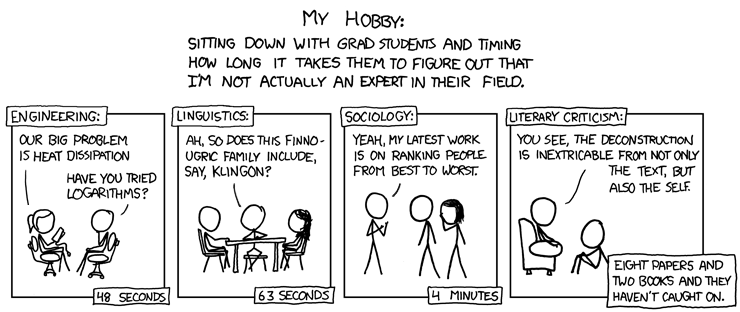
\includegraphics[width=\linewidth]{figures/sci_faking}
\caption{fig:faking}
\end{figure}

\paragraph{Specialized Vocabularies Define Fields of Study}

First, scientific documents are unique because unlike ``general'' documents,
their vocabulary is precise and carefully measured.  ``Resistance'', ``splice'',
``utilization'', and ``demand'' are common words with radically different
meanings when used in specialized, technical contexts.  Their use is a
shibboleth whose use shows that you a member of a specific discipline
(Figure~\ref{fig:faking}).  Thus, the ability of topic models to capture
patterns of word usage also captures community and affiliation; this goes well
beyond the thematic uses of topic models described in previous chapters.

\paragraph{Scientific Documents Innovate}

As any researcher will tell you, not every scientific publication is innovative;
the sad truth is that most are not.  However, some scientific monographs are
Earth shattering (hopefully just figuratively).  Unlike the other domains we've
discussed, scientific documents are not just \emph{reports} of news or events;
they actually \emph{are the news}.

What makes the analysis of scientific document collections both challenging and
interesting is that innovation is hard to detect and hard to attribute.
Einstein's groundbreaking 1905 papers were not fully recognized until many years
later; important ideas are often proposed by an obscure researcher but only accepted
once popularized and supported by another research; which document (researcher)
in this case was the true source of the innovation?  As we will see in this
chapter, topic models can help answer this question.

\paragraph{Policy Makers Understanding Scientific Documents}

Understanding scientific publications is important for funding agencies,
lawmakers, and the public.  Government funding of science can create jobs,
improve culture, and is an important form of international ``soft power''.
However, knowing which research to fund is difficult, as the nature of science
means that fields constantly change, which precludes rigid
classifications~\citep{szostak-04}.  One challenge of modeling scientific
documents is modeling how fields change over time; the static models we've
discussed thus far are not always appropriate.

\section{Understanding Fields of Studies}

Topics can correspond to rough fields of studies.  This insight was
noted early in the development of topic models~\citep{griffiths-04}.

Topic models can show where official designations or labels conflict
with reality~\citep{talley-11}.

Where we have labels we trust, we can use them to constrain
topics~\citep{ramage-09}.

But if the labels are two coarse, we can use topic models to refine
them or organize the\citep{Nguyen:Boyd-Graber:Resnik:Chang-2014}

\section{How Fields Change over Time}
\label{sec:science_fields}

One way that science is unique from the fields discussed in the
previous chapters is that it is part of a continuous dialog.  Each
paper in its own way stands on the shoulders of giants. Topic models
for science thus need to be aware of the connections between documents
over time.

One of the first techniques to do this viewed topics as subtly
changing each year~\citep{blei-06b}.  Example of physics going from
ether to accelerators.

The flipping of a calendar page does not rule science, however;
changes can happen at any time~\citep{wang-06,wang-08}.

\section{Innovation}

Fields change because innovation happens.  Identifying who is
responsible for the changes can find who is ``winning'' the race to
introduce, explain, and popularize new ideas.

From an institutional perspective, we can see which universities have
research portfolios that look like the future~\citep{ramage-10}.

This is important not just for science historians but also for policy
makers~\citep{largent-12}.

Institutions are where science happens, but the true drivers of
innovation are individual researchers who present their papers as the
place where research happens~\citep{gerrish-10}.
